\subsection{Probleem van de dinerende filosofen}

Beginsituatie:

\begin{itemize}
\item filosofen
\item 1  tafel met 5 borden en 5 vorken
\item Spaghetti wordt gegeten met de twee vorken naast het bord 
\end{itemize}

Beperkingen:

\begin{itemize}
\item Moet voldoen aan wederzijdse uitsluiting: een vork mag niet tegelijkertijd door meerdere filosofen worden gebruikt.
\item Geen deadlock of(letterlijke) uithongering mag er gebeuren.
\end{itemize}

\subsubsection{Een oplossing met semaforen }

Een eerste oplossing:
 
 
 
 \begin{figure}[htp]
    \centering
            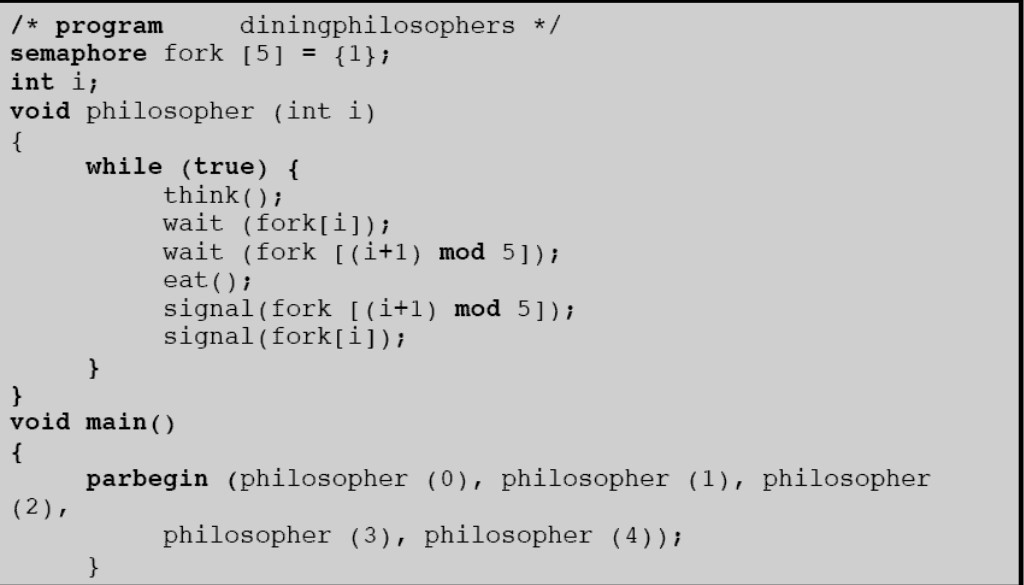
\includegraphics[width=4in]{img/oplossingsemafoor.jpg}
        \caption{Voorbeeld geen deadlock}
    \label{fig:Voorbeeld geen deadlock}
\end{figure}

Bovenstaande oplossing leidt tot een deadlock.




Uitsluiting van deadlock kan door het aantal processen aan tafel te beperken tot aantal processen – 1 => er is minstens 1 proces dat de nodige bronnen kan gebruiken en volledig kan uitgevoerd worden.

 \begin{figure}[htp]
    \centering
            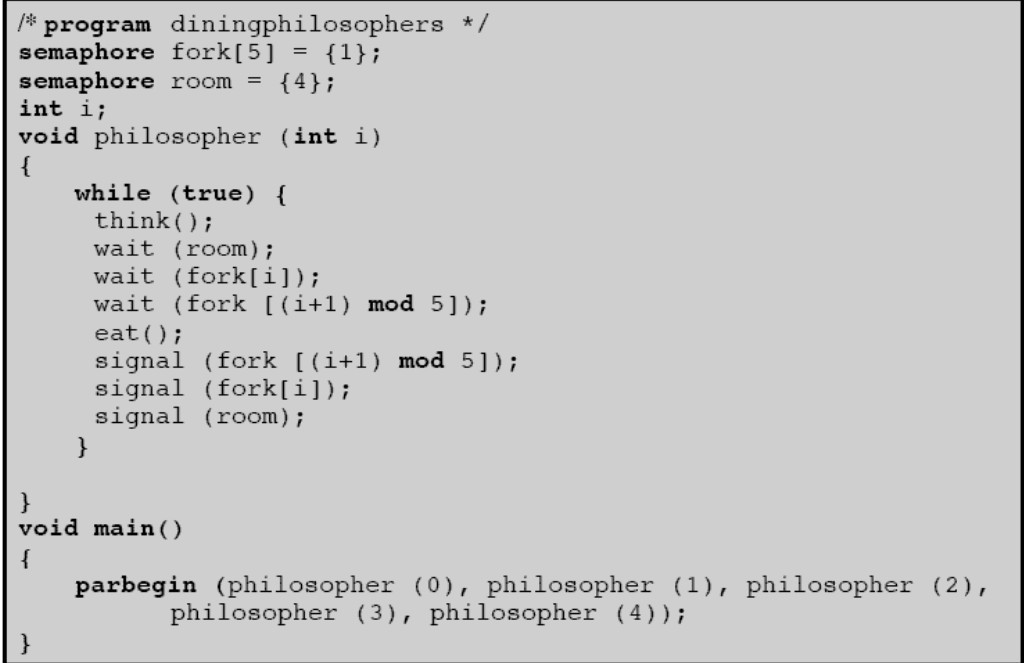
\includegraphics[width=4in]{img/oplossingsemafoor2.jpg}
        \caption{Voorbeeld geen deadlock}
    \label{fig:Voorbeeld geen deadlock}
\end{figure}

\subsubsection{Een oplossing met een monitor}
We hebben een vector met 5 conditievariabelen: 1 per vork en een vector met 5 booleans: na te gaan of een vork beschikbaar is, als dat niet is, dan moet het proces in de wachtrij van die vork.